\documentclass[12pt]{article}
\usepackage{graphicx}
\begin{document}
\section{Task 1}

\subsection{Task A}
Prepare a use case diagram for the following description:  \\

"A student can check a timetable of the lessons and its own results in the university system.  To use these services the student needs to authorize in the system. The student can add its comment to the timetable, if necessary." 
\\
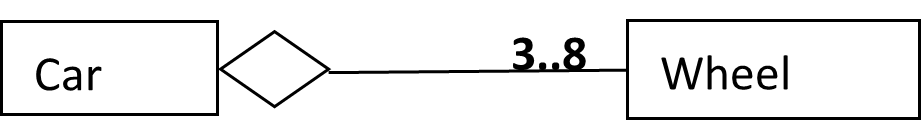
\includegraphics[width=\textwidth]{1A}

\subsection{Task B}
Propose different ways of modelling of a student authorization (different diagrams).  \\ 
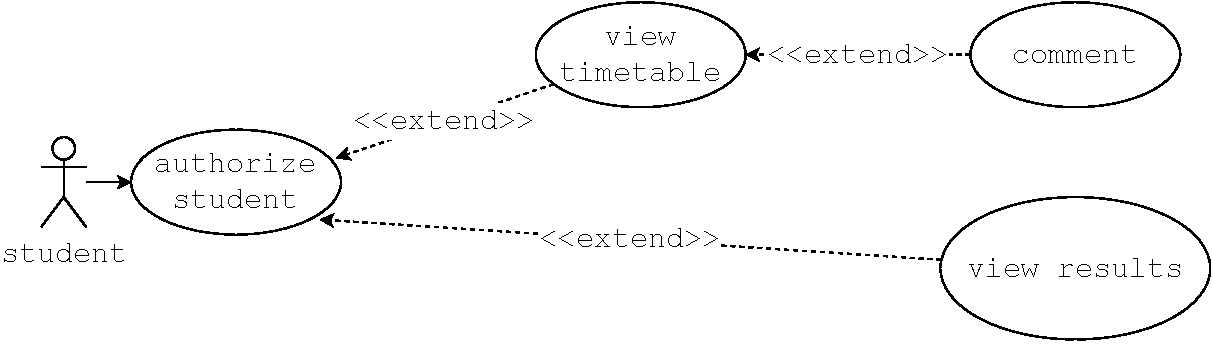
\includegraphics[width=\textwidth]{1B}


\newpage
\section{Task 2}
Categorize the following relationships into \textbf{generalization},  \textbf{aggregation}, or  \textbf{association}. Draw an appropriate  \textbf{class diagram}. There could be more than one solution if applicable. 


\subsection{A dining philosopher is using a fork.}
Dining philosopher is using \textbf{exactly} one fork and one fork is used \textbf{exactly} by one philosopher. \\ 
This is \textbf{association}, this is not aggregation as fork is not a part of philosopher, neither philosopher part of fork, and this is not generalization as philosopher is not a kind of fork and fork is not a kind of philosopher.
\\ 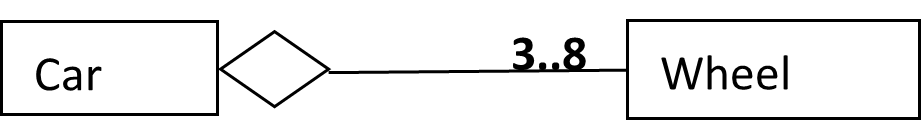
\includegraphics[width=\textwidth]{31}
\subsection{A file is an ordinary file or a directory file. } 
This is \textbf{generalization}, ordinary file is a kind of file, also directory is a kind of file, this is not aggregation as ordinary/directory file is not part of file.
\\ 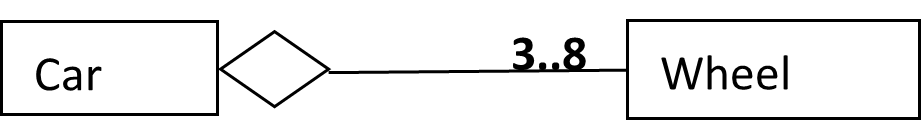
\includegraphics[width=\textwidth]{32}

\subsection{Files contain records.}
This is \textbf{aggregation}, records are part of files, this is not generalization as records are not kind of file. 
\\ 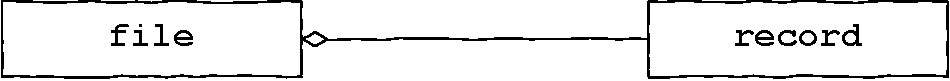
\includegraphics[width=\textwidth]{33}


\subsection{A polygon is composed of an ordered set of points. }
This is \textbf{aggregation}, points are part of polygon, this is not generalization as points are not kind of polygon. 
\\ 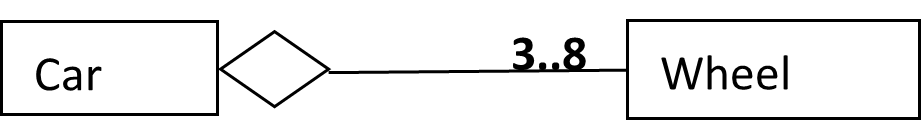
\includegraphics[width=\textwidth]{34}

\subsection{A person uses a computer language on a project. }
This is \textbf{association}, this is not aggregation as computer language is not a part of person, neither person part of computer language, and this is not generalization as person is not a kind of computer language and computer language is not a kind of person.
\\ 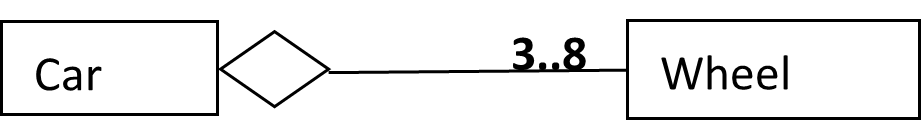
\includegraphics[width=\textwidth]{35}
\subsection{A route connects two cities }
This is \textbf{association}, cities are associated through route.
\\ 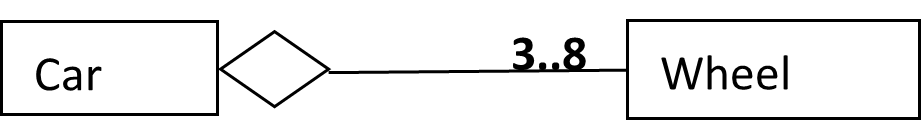
\includegraphics[width=\textwidth]{36}


\subsection{Modems and keyboards are input/output devices. }
This is \textbf{generalization}, Modems and keyboards are kind of input/output devices, this is not aggregation as modems/keyboards are not part of input/output devices
\\ 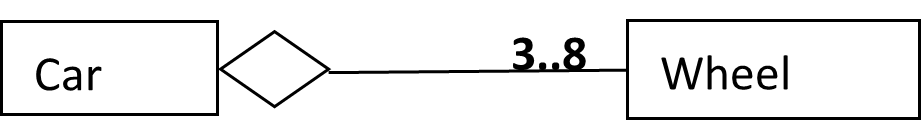
\includegraphics[width=\textwidth]{37}
\section{Task 3}
Are the following sentences consistent with the given class diagram (Explain)?
\\
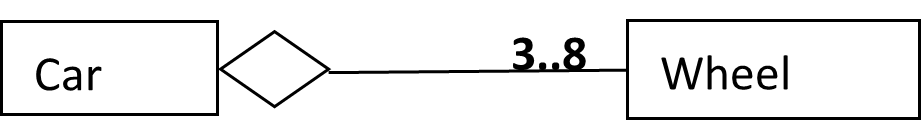
\includegraphics[width=\textwidth]{Class1_103.png}

\paragraph{“John’s car has 10 wheels, including the spares.” }
It is \textbf{not consistent} as there is maximum of \textbf{8} wheels on a car.
\paragraph{“Each car has at least one wheel.” }
It is \textbf{consistent} and true always, as each car has minimum of \textbf{3} wheels on a car
\paragraph{“In my car, there are two wheels on the left side and two wheels on the right side”  } 
It is \textbf{consistent}, this particular car contains wheels in amount between minimum and maximum, we do not care about the position of those wheels in our class diagram.

\paragraph{Draw an exemplary object diagram for the class diagram. }
\section{Task 4}
Prepare a class diagram based on the following description of a card-playing program. 
\\
“Deck, hand, discard pile, and draw pile are collection of cards. The initial size of the hand depends on the type of game. The collection of cards consists of an ordered set of cards. A card can be displayed and discarded. Each card is characterized by its suit and rank. At the beginning of the game the collection of cards is initialized. The cards on the deck can be shuffled.” 
\\
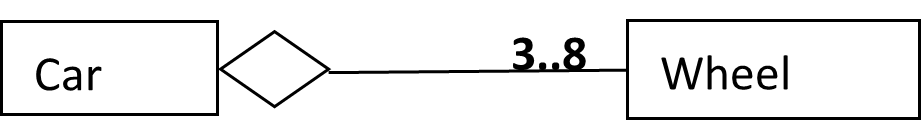
\includegraphics[width=\textwidth]{4}



\end{document}